\documentclass[11pt, a4paper]{article}

% --- PREAMBLE ---
\usepackage[a4paper, top=2.5cm, bottom=2.5cm, left=2.5cm, right=2.5cm]{geometry}
\usepackage{amsmath}
\usepackage{amssymb}
\usepackage{graphicx}
\usepackage{physics}
\usepackage{tikz}
\usepackage{tikz-feynman}
\usepackage{float}


% Custom commands
\newcommand{\Lscr}{\mathcal{L}}
\newcommand{\be}{\begin{equation}}
\newcommand{\ee}{\end{equation}}

% --- DOCUMENT ---
\begin{document}

\title{Solutions to Physics 151 Mid-Term Examination\\
\large Introduction to Quantum Field Theory}
\author{Xiaoyang Zheng}
\date{\today}
\maketitle

% --- PROBLEM 1 ---
\section{Problem 1: Vacuum Energy in $\phi^4$ Theory}

We consider the action for a real scalar field $\phi(x^\mu)$ in four spacetime dimensions:
\be
S=\int d^{4}x\left\{\frac{1}{2}(\partial\phi)^{2}-\frac{1}{2}m^{2}\phi^{2}-\frac{1}{4!}\lambda\phi^{4}\right\}.
\ee

\subsection{Part (i) \& (ii): Connected Vacuum Diagrams and Symmetry Factors}

Vacuum diagrams are Feynman diagrams with no external legs. We construct these by contracting all fields at interaction vertices. The symmetry factor $S$ of a diagram is defined as the number of ways the diagram remains invariant under permutations of its elements.

\subsubsection*{Order $\mathbf{\lambda^1}$: Figure-Eight Diagram}

\textbf{Topology:} At first order in $\lambda$, there will be a single 4-point vertex from the $\phi^4$ interaction. All four fields must be contracted in pair to form two loops sharing a common vertex, creating a "8" structure.

\textbf{Diagram:} Two propagator loops attached to the same vertex.

\begin{figure}[H]
    \centering
    
\includegraphics[width=0.1\textwidth]{1-1.jpg}
    \caption{Vacuum diagram (order $\lambda^1$).}
    \label{fig:figure8}
\end{figure}

\textbf{Symmetry Factor:} We count all permutations leaving the diagram invariant:
\begin{itemize}
    \item Interchange the two loops: factor of 2
    \item Within each loop, the two propagators can be swapped: factor of $2 \times 2 = 4$
\end{itemize}
Total symmetry factor: $S = 2 \times 2 \times 2 = 8$.

\subsubsection*{Order $\mathbf{\lambda^2}$: Two Distinct Topologies}

At second order in $\lambda$, we have two vertices with eight half-lines total. All must be contracted to form vacuum diagrams.

\textbf{ Diagram A:}

\textbf{Topology:} Two vertices connected by two propagators, with each vertex having an additional self-loop.

\textbf{Diagram:} 
\begin{figure}[H]
    \centering
    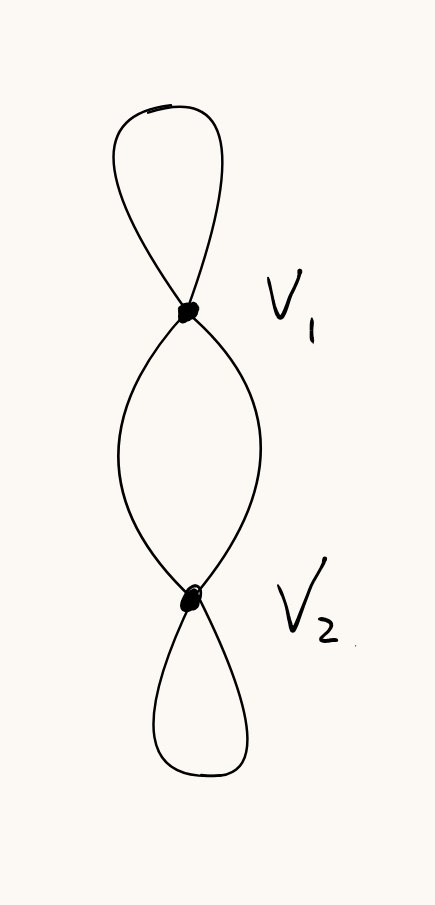
\includegraphics[width=0.1\textwidth]{2-1.jpg}
    \caption{Vacuum diagram A (order $\lambda^2$).}
    \label{fig:figureooo}
\end{figure}

\textbf{Symmetry Factor:}
\begin{itemize}
    \item Interchange the two vertices: factor of 2
    \item Swap the two propagators connecting the vertices: factor of 2
    \item Swap the two propagators in the loop at vertex 1: factor of 2
    \item Swap the two propagators in the loop at vertex 2: factor of 2
\end{itemize}
Total symmetry factor: $S = 2^4 = 16$.


\textbf{(b) Diagram B:}

\textbf{Topology:} Two vertices connected by four parallel propagators (no self-loops).

\textbf{Diagram:}
\begin{figure}[H]
    \centering
    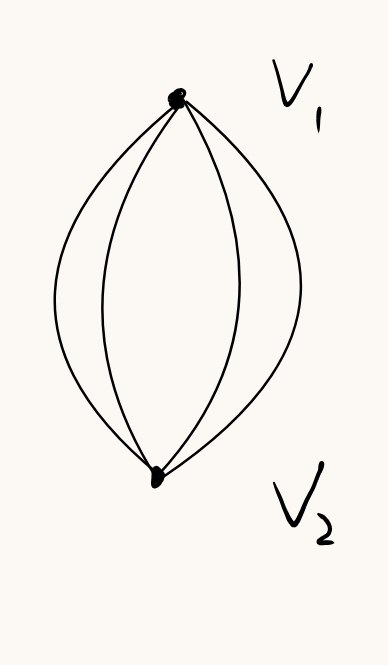
\includegraphics[width=0.1\textwidth]{2-2.jpg}
    \caption{Vacuum diagram B (order $\lambda^2$).}
    \label{fig:figurebbb}
\end{figure}

\textbf{Symmetry Factor:}
\begin{itemize}
    \item Interchange the two vertices: factor of 2
    \item Permute all four propagators: factor of $4! = 24$
\end{itemize}
Total symmetry factor: $S = 2 \times 24 = 48$.


\subsection{Part (iii): Mass Dimension of $\lambda$ in $d$ Dimensions}

In natural units ($\hbar = c = 1$), the action $S$ must be dimensionless. We work in $d = D+1$ spacetime dimensions.

\begin{itemize}
    \item The integration measure $d^dx$ has dimension $[d^dx] = -d$ (since $[x] = -1$ in energy units).
    \item The Lagrangian density must satisfy $[\Lscr] = d$ to make $S = \int d^dx\, \Lscr$ dimensionless.
    \item From the kinetic term $(\partial_\mu\phi)^2$: with $[\partial_\mu] = 1$, we have
    \be
    [(\partial\phi)^2] = 2([\partial] + [\phi]) = 2(1 + [\phi]) = d.
    \ee
    This gives $[\phi] = \frac{d-2}{2}$.
    \item From the interaction term $\lambda\phi^4$:
    \be
    [\lambda] + 4[\phi] = d \implies [\lambda] = d - 4[\phi] = d - 4\cdot\frac{d-2}{2} = d - 2(d-2) = 4 - d.
    \ee
\end{itemize}

\textbf{Summarize:} In $d$ spacetime dimensions, $[\lambda] = 4 - d$. Specifically:
\begin{itemize}
    \item In $d = 4$: $[\lambda] = 0$ (dimensionless, marginal coupling)
    \item In $d < 4$: $[\lambda] > 0$ (relevant coupling)
    \item In $d > 4$: $[\lambda] < 0$ (irrelevant coupling)
\end{itemize}

\subsection{Part (iv): Mass Dimension of $g$ for $\phi^3$ Interaction}

If we add a cubic interaction $g\phi^3$ to the Lagrangian, we apply the same dimensional analysis:

\textbf{In $d = 4$ dimensions:}
\be
[g\phi^3] = [g] + 3[\phi] = 4 \implies [g] = 4 - 3 \times 1 = 1.
\ee

\textbf{General formula in $d$ dimensions:}
\be
[g] = d - 3[\phi] = d - 3 \cdot \frac{d-2}{2} = d - \frac{3(d-2)}{2} = \frac{2d - 3d + 6}{2} = \frac{6-d}{2}.
\ee

In $d=4$ dimensions, $[g] = 1$ (dimension of mass). In general $d$ dimensions, $[g] = \frac{6-d}{2}$.

% --- PROBLEM 2 ---
\section{Problem 2: Scaling Dimensions of Free Fields}

We compare the scaling properties of relativistic and non-relativistic free scalar field theories in $d = D+1$ spacetime dimensions.

\subsection{Part (i): Scaling Dimension of Relativistic Field $\phi$}

The relativistic free field has action:
\be
S_{\text{rel}}=\frac{1}{2}\int d^{d}x\,(\partial_{\mu}\phi)(\partial^{\mu}\phi).
\ee

\textbf{Dimensional Analysis:}
\begin{itemize}
    \item The measure $d^dx$ has dimension $[d^dx] = -d$.
    \item For dimensionless action, we require $[\Lscr_{\text{rel}}] = d$.
    \item The derivative has $[\partial_\mu] = 1$ (energy units).
    \item From $[(\partial\phi)^2] = d$, we obtain:
    \be
    2([\partial] + [\phi]) = d \implies 2(1 + [\phi]) = d \implies [\phi] = \frac{d-2}{2}.
    \ee
\end{itemize}

In $d$ spacetime dimensions, the relativistic scalar field has scaling dimension 

$$[\phi] = \frac{d-2}{2}$$

For example, in $d = 4$: $[\phi] = 1$ (dimension of mass).

\subsection{Part (ii): Scaling Dimension of Non-Relativistic Field $\Phi$}

The non-relativistic (Lifshitz) scalar has action:
\be
S_{\text{nonrel}}=\frac{1}{2}\int dt\, d^{D}x\left\{(\dot{\Phi})^{2}-(\partial_{i}\partial_{i}\Phi)(\partial_{j}\partial_{j}\Phi)\right\}.
\ee

The action $S_{\text{nonrel}}$ exhibits anisotropic scaling where time and space scale differently.

The two kinetic terms must have the same dimension. Setting $[\partial_t] = 1$ and $[\partial_i] = z$, because $E = -i\partial_t$:
\be
[(\dot{\Phi})^2] = [(\nabla^2\Phi)^2] \implies 2(1+[\Phi]) = 2(2z+[\Phi]) \implies z = 1/2.
\ee
This implies $[t] = -1$ and $[x^i] = -1/2$.

\textbf{Field Dimension:} The action must be dimensionless. The integration measure gives $[dt\,d^Dx] = -1 - D/2$, so we need $[\Lscr_{\text{nonrel}}] = 1 + D/2$. Equating this to the dimension of the time-derivative term:
\be
2(1+[\Phi]) = 1 + D/2 \implies [\Phi] = \frac{D-2}{4}.
\ee

he non-relativistic Lifshitz scalar has scaling dimension $[\Phi] = \frac{D-2}{4}$ in $d = D+1$ dimensions.

For example, in $d = 4$ (i.e., $D = 3$): $[\Phi] = 1/4$.

\subsection{Part (iii): Feynman Propagator for the Lifshitz Scalar}

\textbf{Derivation from the Equation of Motion:}

The Euler-Lagrange equation from $S_{\text{nonrel}}$ gives:
\be
\frac{\delta S}{\delta\Phi} = 0 \implies -\partial_t^2\Phi + \nabla^4\Phi = 0.
\ee

In momentum space with Fourier transform $\Phi(t,\vec{x}) = \int \frac{d\omega\,d^Dk}{(2\pi)^{D+1}} e^{-i\omega t + i\vec{k}\cdot\vec{x}} \tilde{\Phi}(\omega,\vec{k})$:
\begin{itemize}
    \item $\partial_t \to -i\omega$
    \item $\nabla^2 \to -k^2$ where $k = |\vec{k}|$
\end{itemize}

The equation becomes:
\be
\omega^2 - k^4 = 0.
\ee

\textbf{Propagator with $i\epsilon$ Prescription:}

The Feynman propagator is obtained by inverting the kinetic operator with the standard $i\epsilon$ prescription for time-ordering:
\be
D_F(\omega, \vec{k}) = \frac{i}{\omega^2 - k^4 + i\epsilon}.
\ee

\textbf{Normalization:} The numerator is normalized to $i$ (not $-i$) for consistency with the canonical commutation relations. The scalar field $\Phi$ has a single degree of freedom (one independent polarization), justifying the simple numerator.

\textbf{Position Space Form:}
\be
D_F(t-t', \vec{x}-\vec{x}') = \int \frac{d\omega\,d^Dk}{(2\pi)^{D+1}} \frac{i\,e^{-i\omega(t-t') + i\vec{k}\cdot(\vec{x}-\vec{x}')}}{\omega^2 - k^4 + i\epsilon}.
\ee

The Feynman propagator is $D_F(\omega,\vec{k}) = \frac{i}{\omega^2 - k^4 + i\epsilon}$, with numerator normalized to unity (times $i$) reflecting the single polarization of the scalar field.

% --- PROBLEM 3 ---
\section{Problem 3: Renormalization Group Flow in Lifshitz Theory}

We extend the non-relativistic Lifshitz scalar theory by adding two Gaussian (quadratic) terms:
\be
\hat{S}_{\text{nonrel}}=\frac{1}{2}\int dt\, d^{3}x\left\{(\dot{\Phi})^{2}-(\partial_{i}\partial_{i}\Phi)(\partial_{j}\partial_{j}\Phi)-c^{2}(\partial_{i}\Phi)(\partial_{i}\Phi)-m^{2}\Phi^{2}\right\}.
\ee

We now analyze this theory in $d = 4$ spacetime dimensions (i.e., $D = 3$ spatial dimensions) from the perspective of renormalization group (RG) flow.

\subsection{Part (i): Relevance of the Couplings $c^2$ and $m^2$}

From Problem 2(ii), we established that for the Lifshitz scalar in $D$ spatial dimensions:
\begin{itemize}
    \item Dynamical exponent: $z = 2$
    \item Field dimension: $[\Phi] = \frac{D-2}{4}$
    \item Lagrangian density dimension: $[\Lscr] = 2 + D$
\end{itemize}

For $D = 3$, we have:
\begin{itemize}
    \item $[\Phi] = \frac{3-2}{4} = \frac{1}{4}$
    \item $[\Lscr] = 2 + 3 = 5$
    \item $[\partial_i] = 1$ (spatial derivative)
\end{itemize}

\textbf{Dimension of $m^2$:}

From the mass term $m^2\Phi^2$, requiring $[m^2\Phi^2] = 5$:
\be
[m^2] + 2[\Phi] = 5 \implies [m^2] + 2 \times \frac{1}{4} = 5 \implies [m^2] = 5 - \frac{1}{2} = \frac{9}{2}.
\ee

Since $[m^2] = \frac{9}{2} > 0$, the coupling $m^2$ is \textbf{relevant}.

\textbf{Dimension of $c^2$:}

From the gradient term $c^2(\partial_i\Phi)^2$, requiring $[c^2(\partial_i\Phi)^2] = 5$:
\be
[c^2] + 2([\partial_i] + [\Phi]) = 5 \implies [c^2] + 2\left(1 + \frac{1}{4}\right) = 5 \implies [c^2] + \frac{5}{2} = 5.
\ee
Therefore:
\be
[c^2] = 5 - \frac{5}{2} = \frac{5}{2}.
\ee

Since $[c^2] = \frac{5}{2} > 0$, the coupling $c^2$ is also \textbf{relevant}.

Both couplings are \textbf{relevant}, meaning they grow under RG flow toward the infrared (low energies).

\subsection{Part (ii): Qualitative RG Flow Patterns}

\textbf{Fixed Point Structure:}

The point $(c^2, m^2) = (0, 0)$ corresponds to the pure Lifshitz theory without the additional perturbations. This is a critical point of the RG flow.

\textbf{Flow Behavior:}
\begin{itemize}
    \item Since both $c^2$ and $m^2$ are relevant couplings with positive mass dimensions, they grow as we flow toward the infrared (decreasing energy scale).
    \item The origin $(0,0)$ is an \textbf{ultraviolet (UV) unstable fixed point}—the Lifshitz fixed point is attractive in the UV direction but repulsive in the IR.
    \item Starting from any point $(c^2, m^2) \neq (0,0)$ in the parameter space, RG flow moves away from the origin as energy decreases.
\end{itemize}

\textbf{Flow Pattern Description:}
\begin{itemize}
    \item Near the origin, both couplings increase under RG flow toward lower energies.
    \item The flow is radially outward from the Lifshitz point $(0,0)$.
    \item The eigendirections of the flow are determined by the RG eigenvalues $\lambda_{c^2} = [c^2] = 5/2$ and $\lambda_{m^2} = [m^2] = 9/2$.
    \item Since $\lambda_{m^2} > \lambda_{c^2}$, the $m^2$ direction is "more relevant" and grows faster.
\end{itemize}

The RG flow exhibits a UV-stable (IR-unstable) fixed point at the origin. All flow lines move radially outward from $(0,0)$ toward the infrared, with $m^2$ growing faster than $c^2$.

\subsection{Part (iii): Emergent Relativistic Lorentz Symmetry}

\textbf{Question:} Is there an RG fixed point exhibiting emergent relativistic symmetry?

\textbf{Analysis:}

For relativistic symmetry to emerge, the dispersion relation must become $\omega^2 \sim k^2$ (light-cone structure) rather than $\omega^2 \sim k^4$ (Lifshitz scaling).

In the full action $\hat{S}_{\text{nonrel}}$, the equation of motion in momentum space is:
\be
\omega^2 - k^4 - c^2 k^2 - m^2 = 0.
\ee

At high momenta (UV limit, $k \to \infty$):
\begin{itemize}
    \item The $k^4$ term dominates: $\omega^2 \approx k^4$, giving Lifshitz scaling.
    \item This corresponds to the Lifshitz fixed point $(c^2, m^2) = (0,0)$.
\end{itemize}

At low momenta (IR limit, $k \to 0$):
\begin{itemize}
    \item If $c^2 > 0$ and $c^2 \gg m^2/k^2$, the $c^2 k^2$ term dominates over both $k^4$ and $m^2$.
    \item The dispersion becomes $\omega^2 \approx c^2 k^2$, which is relativistic with effective "speed of light" $c$.
    \item The $k^4$ term becomes negligible in comparison (higher-derivative/irrelevant operator).
\end{itemize}

\textbf{Fixed Point Location:}

The emergent relativistic symmetry does not appear at a traditional fixed point but rather in the \textbf{infrared regime} where $c^2$ and $m^2$ have grown large.

More precisely, we can identify an effective IR theory:
\begin{itemize}
    \item In the regime where $c^2 k^2 \gg k^4$ and $m^2 \ll c^2 k^2$, the theory reduces to:
    \be
    S_{\text{eff}} \approx \frac{1}{2}\int dt\,d^3x\left\{(\dot{\Phi})^2 - c^2(\partial_i\Phi)^2\right\},
    \ee
    which is manifestly relativistic with Lorentz symmetry and speed $c$.
\item This corresponds to a "Lorentz-invariant Gaussian fixed point" in the extended theory.
\end{itemize}

So yes, emergent relativistic Lorentz symmetry appears in the \textbf{infrared (low-energy) limit}. As $c^2$ grows relevant under RG flow, the theory flows toward an effective relativistic theory where the dispersion relation becomes $\omega^2 = c^2 k^2 + m^2$. The Lifshitz $k^4$ term becomes an irrelevant higher-derivative correction in this regime. 

This is an example of \textbf{emergent Lorentz symmetry}, where a fundamentally non-relativistic UV theory flows to a relativistic IR fixed point. The phenomenon occurs not at the UV Lifshitz point $(0,0)$, but in the IR regime where $c^2 \to \infty$ (in dimensionless RG flow).

% --- PROBLEM 4 ---
\section{Problem 4: Propagators and Green's Functions}

We return to the relativistic $\phi^4$ theory from Problem 1, focusing on tree-level propagators.

\subsection{Part (i): Advanced and Feynman Propagators in Momentum Space}

The free Klein-Gordon equation is:
\be
(\Box + m^2)\phi(x) = 0 \quad \text{where} \quad \Box = \partial_\mu\partial^\mu.
\ee

The propagators are Green's functions satisfying:
\be
(\Box_x + m^2)D(x-y) = -i\delta^{(4)}(x-y).
\ee

In momentum space, with Fourier convention:
\be
D(x-y) = \int \frac{d^4k}{(2\pi)^4} e^{-ik\cdot(x-y)} \tilde{D}(k),
\ee
we have $\Box \to -k^2 = -k^\mu k_\mu = -(k_0^2 - \vec{k}^2)$.

The equation becomes:
\be
(-k^2 + m^2)\tilde{D}(k) = -i \implies (k^2 - m^2)\tilde{D}(k) = i.
\ee

\textbf{(a) Feynman Propagator $D_F(x-y)$:}

The Feynman propagator time-orders the fields and uses the $+i\epsilon$ prescription in the denominator to specify contour integration around the poles:
\be
\boxed{D_F(x-y) = \int \frac{d^4k}{(2\pi)^4} \frac{i\,e^{-ik\cdot(x-y)}}{k^2 - m^2 + i\epsilon}}
\ee

Alternatively, in terms of energy-momentum:
\be
D_F(x-y) = \int \frac{d^4k}{(2\pi)^4} \frac{i\,e^{-ik^0(x^0-y^0) + i\vec{k}\cdot(\vec{x}-\vec{y})}}{k_0^2 - \vec{k}^2 - m^2 + i\epsilon}.
\ee

The $i\epsilon$ prescription places both poles slightly below the real axis in the complex $k^0$ plane, ensuring causality and correct time-ordering.

\textbf{(b) Advanced Propagator $D_A(x-y)$:}

The advanced propagator vanishes for $x^0 < y^0$ and propagates disturbances backward in time. The $i\epsilon$ prescription is modified:
\be
\boxed{D_A(x-y) = \int \frac{d^4k}{(2\pi)^4} \frac{i\,e^{-ik\cdot(x-y)}}{k^2 - m^2 - i\epsilon}}
\ee

Equivalently:
\be
D_A(x-y) = \int \frac{d^4k}{(2\pi)^4} \frac{i\,e^{-ik^0(x^0-y^0) + i\vec{k}\cdot(\vec{x}-\vec{y})}}{k_0^2 - \vec{k}^2 - m^2 - i\epsilon}.
\ee

The sign flip in $i\epsilon$ places both poles slightly above the real $k^0$ axis, giving the advanced boundary condition.


\subsection{Part (ii): Differential Equation Satisfied by the Propagators}

\textbf{Question:} Do $D_F(x-y)$ and $D_A(x-y)$ satisfy the same differential equation?

\textbf{Yes}, both propagators satisfy the same inhomogeneous Klein-Gordon equation:
\be
\boxed{(\Box_x + m^2)D(x-y) = -i\delta^{(4)}(x-y)}
\ee

\textbf{Proof:}

We apply the Klein-Gordon operator to either propagator in momentum space:
\be
(\Box_x + m^2)D(x-y) = \int \frac{d^4k}{(2\pi)^4} (-k^2 + m^2) \tilde{D}(k) e^{-ik\cdot(x-y)}.
\ee

For both the Feynman and advanced propagators:
\be
\tilde{D}(k) = \frac{i}{k^2 - m^2 \pm i\epsilon},
\ee
we compute:
\be
(-k^2 + m^2)\tilde{D}(k) = (-(k^2 - m^2)) \cdot \frac{i}{k^2 - m^2 \pm i\epsilon}.
\ee

In the limit $\epsilon \to 0^+$ (after integration), this becomes:
\be
= \frac{-(k^2-m^2) \cdot i}{k^2 - m^2 \pm i\epsilon} \to -i,
\ee
independent of the sign of $i\epsilon$. The $\pm i\epsilon$ prescription affects \emph{how} we integrate (contour choice), not the formal algebraic result.

Therefore:
\be
(\Box_x + m^2)D(x-y) = \int \frac{d^4k}{(2\pi)^4} (-i) e^{-ik\cdot(x-y)} = -i\delta^{(4)}(x-y).
\ee

So both $D_F$ and $D_A$ are Green's functions for the same differential operator $(\Box + m^2)$, satisfying identical equations. They differ only in their boundary conditions (time-ordering vs. advanced causality), which is encoded in the $i\epsilon$ prescription and manifests in different analytic properties, but not in the formal differential equation itself.



\end{document}

